\let\negmedspace\undefined
\let\negthickspace\undefined
\documentclass[journal]{IEEEtran}
\usepackage[a5paper, margin=10mm, onecolumn]{geometry}
\usepackage{tfrupee}

\setlength{\headheight}{1cm}
\setlength{\headsep}{0mm}
\usepackage{gvv-book}
\usepackage{gvv}
\usepackage{cite}
\usepackage{amsmath,amssymb,amsfonts,amsthm}
\usepackage{algorithmic}
\usepackage{graphicx}
\usepackage{textcomp}
\usepackage{xcolor}
\usepackage{txfonts}
\usepackage{listings}
\usepackage{enumitem}
\usepackage{mathtools}
\usepackage{gensymb}
\usepackage{comment}
\usepackage[breaklinks=true]{hyperref}
\usepackage{tkz-euclide}
\def\inputGnumericTable{}
\usepackage[latin1]{inputenc}
\usepackage{color}
\usepackage{array}
\usepackage{longtable}
\usepackage{calc}
\usepackage{multirow}
\usepackage{hhline}
\usepackage{ifthen}
\usepackage{lscape}
\usepackage{booktabs}
\usepackage{tikz}
\usetikzlibrary{arrows.meta,angles,quotes}

\begin{document}

\bibliographystyle{IEEEtran}
\vspace{3cm}

\title{2.6.23}
\author{AI25BTECH11014 - Gooty Suhas}
{\let\newpage\relax\maketitle}

\renewcommand{\thefigure}{\theenumi}
\renewcommand{\thetable}{\theenumi}
\setlength{\intextsep}{10pt}
\numberwithin{equation}{enumi}
\numberwithin{figure}{enumi}
\renewcommand{\thetable}{\theenumi}

\section*{\large\textbf{Problem}}
\vspace{0.5cm}

Find the area of a triangle whose vertices are given in 3D space as:
\[
\vec{A} = \myvec{1 \\ 1 \\ 1}, \quad
\vec{B} = \myvec{1 \\ 2 \\ 3}, \quad
\vec{C} = \myvec{2 \\ 3 \\ 1}
\]
We will compute the area using the formula:
\[
\text{Area} = \frac{1}{2} \left\| (\vec{B} - \vec{A}) \times (\vec{C} - \vec{A}) \right\|
\]

\section*{\large\textbf{Solution}}
\vspace{0.5cm}

\subsection*{Step 1: Compute Vectors}
\[
\vec{B} - \vec{A} = \myvec{1 \\ 2 \\ 3} - \myvec{1 \\ 1 \\ 1} = \myvec{0 \\ 1 \\ 2}
\]
\[
\vec{C} - \vec{A} = \myvec{2 \\ 3 \\ 1} - \myvec{1 \\ 1 \\ 1} = \myvec{1 \\ 2 \\ 0}
\]

\subsection*{Step 2: Cross Product}
\[
(\vec{B} - \vec{A}) \times (\vec{C} - \vec{A}) =
\myvec{
(1)(0) - (2)(2) \\
(2)(1) - (0)(0) \\
(0)(2) - (1)(1)
} =
\myvec{-4 \\ 2 \\ -1}
\]

\subsection*{Step 3: Magnitude}
\[
\left\| (\vec{B} - \vec{A}) \times (\vec{C} - \vec{A}) \right\| =
\sqrt{(-4)^2 + 2^2 + (-1)^2} =
\sqrt{16 + 4 + 1} = \sqrt{21}
\]

\subsection*{Step 4: Area}
\[
\text{Area} = \frac{1}{2} \sqrt{21}
\]
\[
\boxed{\text{Area} = \frac{\sqrt{21}}{2}}
\]





\begin{figure}[h!t]
    \centering
    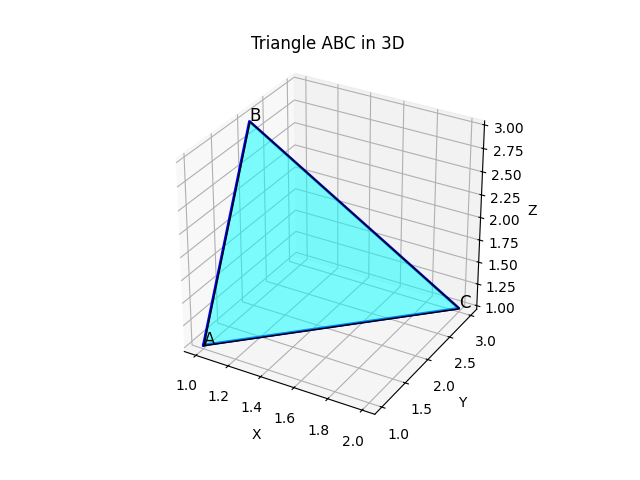
\includegraphics[width=1\linewidth]{Figs/fig1.png}
    \caption{The line}
    \label{fig:fig1}
\end{figure}
















\end{document}
